%% BioMed_Central_Tex_Template_v1.06
%%                                      %
%  bmc_article.tex            ver: 1.06 %
%                                       %

%%IMPORTANT: do not delete the first line of this template
%%It must be present to enable the BMC Submission system to
%%recognise this template!!

%%%%%%%%%%%%%%%%%%%%%%%%%%%%%%%%%%%%%%%%%
%%                                     %%
%%  LaTeX template for BioMed Central  %%
%%     journal article submissions     %%
%%                                     %%
%%          <8 June 2012>              %%
%%                                     %%
%%                                     %%
%%%%%%%%%%%%%%%%%%%%%%%%%%%%%%%%%%%%%%%%%


%%%%%%%%%%%%%%%%%%%%%%%%%%%%%%%%%%%%%%%%%%%%%%%%%%%%%%%%%%%%%%%%%%%%%
%%                                                                 %%
%% For instructions on how to fill out this Tex template           %%
%% document please refer to Readme.html and the instructions for   %%
%% authors page on the biomed central website                      %%
%% http://www.biomedcentral.com/info/authors/                      %%
%%                                                                 %%
%% Please do not use \input{...} to include other tex files.       %%
%% Submit your LaTeX manuscript as one .tex document.              %%
%%                                                                 %%
%% All additional figures and files should be attached             %%
%% separately and not embedded in the \TeX\ document itself.       %%
%%                                                                 %%
%% BioMed Central currently use the MikTex distribution of         %%
%% TeX for Windows) of TeX and LaTeX.  This is available from      %%
%% http://www.miktex.org                                           %%
%%                                                                 %%
%%%%%%%%%%%%%%%%%%%%%%%%%%%%%%%%%%%%%%%%%%%%%%%%%%%%%%%%%%%%%%%%%%%%%

%%% additional documentclass options:
%  [doublespacing]
%  [linenumbers]   - put the line numbers on margins

%%% loading packages, author definitions

%\documentclass[twocolumn]{bmcart}% uncomment this for twocolumn layout and comment line below
\documentclass{doc/template/bmcart-nofigbox}

%%% Load packages
%\usepackage{amsthm,amsmath}
%\RequirePackage{natbib}
%\RequirePackage[authoryear]{natbib}% uncomment this for author-year bibliography
%\RequirePackage{hyperref}
\usepackage[utf8]{inputenc} %unicode support
% \usepackage{fontspec}
% \setmainfont{Cambria}
% \setsansfont{Helvetica}
% \usepackage[applemac]{inputenc} %applemac support if unicode package fails
% \usepackage[latin1]{inputenc} %UNIX support if unicode package fails


%%%%%%%%%%%%%%%%%%%%%%%%%%%%%%%%%%%%%%%%%%%%%%%%%
%%                                             %%
%%  If you wish to display your graphics for   %%
%%  your own use using includegraphic or       %%
%%  includegraphics, then comment out the      %%
%%  following two lines of code.               %%
%%  NB: These line *must* be included when     %%
%%  submitting to BMC.                         %%
%%  All figure files must be submitted as      %%
%%  separate graphics through the BMC          %%
%%  submission process, not included in the    %%
%%  submitted article.                         %%
%%                                             %%
%%%%%%%%%%%%%%%%%%%%%%%%%%%%%%%%%%%%%%%%%%%%%%%%%

\usepackage{graphicx}
\usepackage{placeins}
% \newcommand\includegraphic[1]{}
% \newcommand\includegraphics[1]{}

%%% Put your definitions there:
\startlocaldefs

% Settings to get linked refs.
\PassOptionsToPackage{dvipsnames,svgnames*,x11names*}{xcolor}
\PassOptionsToPackage{unicode=true}{hyperref}
\usepackage{xcolor}
\usepackage{hyperref}
\hypersetup{%
            colorlinks=false,
            linkcolor=Blue,
            citecolor=Blue,
            urlcolor=Blue,
            breaklinks=true
          }

\newcommand{\frnlang}[1]{\textit{#1}}
\newcommand{\taxon}[1]{\frnlang{#1}}
\newcommand{\compcmd}[1]{\texttt{#1}}

\endlocaldefs


%%% Begin ...
\begin{document}

%%% Start of article front matter
\begin{frontmatter}

\begin{fmbox}
\dochead{Research}

%%%%%%%%%%%%%%%%%%%%%%%%%%%%%%%%%%%%%%%%%%%%%%
%%                                          %%
%% Enter the title of your article here     %%
%%                                          %%
%%%%%%%%%%%%%%%%%%%%%%%%%%%%%%%%%%%%%%%%%%%%%%

\title{Changes in the gut microbiota and fermentation products
       associated with enhanced longevity in acarbose-treated mice.}

% TODO: Zenodo the github page?

%%%%%%%%%%%%%%%%%%%%%%%%%%%%%%%%%%%%%%%%%%%%%%
%%                                          %%
%% Enter the authors here                   %%
%%                                          %%
%% Specify information, if available,       %%
%% in the form:                             %%
%%   <key>={<id1>,<id2>}                    %%
%%   <key>=                                 %%
%% Comment or delete the keys which are     %%
%% not used. Repeat \author command as much %%
%% as required.                             %%
%%                                          %%
%%%%%%%%%%%%%%%%%%%%%%%%%%%%%%%%%%%%%%%%%%%%%%

\author[
   addressref={um1},                   % id's of addresses, e.g. {aff1,aff2}
   % corref={},                       % id of corresponding address, if any
   % noteref={},                        % id's of article notes, if any
   email={bjsm@umich.edu}   % email address
]{\inits{BJ}\fnm{Byron J} \snm{Smith}}
\author[
   addressref={um2},                   % id's of addresses, e.g. {aff1,aff2}
   % corref={},                       % id of corresponding address, if any
   % noteref={},                        % id's of article notes, if any
   % email={}   % email address
]{\inits{RA}\fnm{Richard A} \snm{Miller}}
\author[
   addressref={umo},                   % id's of addresses, e.g. {aff1,aff2}
   % corref={},                       % id of corresponding address, if any
   % noteref={},                        % id's of article notes, if any
   % email={}   % email address
]{\inits{AC}\fnm{Aaron C} \snm{Ericsson}}
\author[
   addressref={jl},                   % id's of addresses, e.g. {aff1,aff2}
   % corref={},                       % id of corresponding address, if any
   % noteref={},                        % id's of article notes, if any
   % email={}   % email address
]{\inits{DE}\fnm{David C} \snm{Harrison}}
\author[
   addressref={ut1,ut2,ut3},                   % id's of addresses, e.g. {aff1,aff2}
   % corref={},                       % id of corresponding address, if any
   % noteref={},                        % id's of article notes, if any
   % email={}   % email address
]{\inits{R}\fnm{Randy} \snm{Strong}}
\author[
   addressref={um1,um3},                   % id's of addresses, e.g. {aff1,aff2}
   corref={um3},                       % id of corresponding address, if any
   % noteref={},                        % id's of article notes, if any
   email={schmidti@umich.edu}   % email address
]{\inits{TM}\fnm{Thomas M} \snm{Schmidt}}

%%%%%%%%%%%%%%%%%%%%%%%%%%%%%%%%%%%%%%%%%%%%%%
%%                                          %%
%% Enter the authors' addresses here        %%
%%                                          %%
%% Repeat \address commands as much as      %%
%% required.                                %%
%%                                          %%
%%%%%%%%%%%%%%%%%%%%%%%%%%%%%%%%%%%%%%%%%%%%%%

\address[id=um1]{%                           % unique id
  \orgname{Department of Ecology \& Evolutionary Biology, University of Michigan}, % university, etc
  % \street{Waterloo Road},                     %
  \postcode{48109}                                % post or zip code
  \city{Ann Arbor},                              % city
  \state{MI},
  \cny{USA}                                    % country
}
\address[id=um2]{%                           % unique id
  \orgname{Department of Pathology and Geriatrics Center, University of Michigan}, % university, etc
  % \street{Waterloo Road},                     %
  \postcode{48109}                                % post or zip code
  \city{Ann Arbor},                              % city
  \state{MI},
  \cny{USA}                                    % country
}
\address[id=umo]{%                           % unique id
  \orgname{University of Missouri Metagenomics Center, University of Missouri}, % university, etc
  % \street{},                     %
  \postcode{65201}                                % post or zip code
  \city{Columbia},                              % city
  \state{MO}
  \cny{USA}                                    % country
}
\address[id=jl]{%                           % unique id
  \orgname{The Jackson Laboratory}, % university, etc
  % \street{},                     %
  \postcode{04609}                                % post or zip code
  \city{Bar Harbor},                              % city
  \state{ME}
  \cny{USA}                                    % country
}
\address[id=ut1]{%                           % unique id
  \orgname{Department of Pharmacology, The University of Texas Health Science Center at San Antonio}, % university, etc
  % \street{Waterloo Road},                     %
  \postcode{78229}                                % post or zip code
  \city{San Antonio},                              % city
  \state{TX}
  \cny{USA}                                    % country
}
\address[id=ut2]{%                           % unique id
  \orgname{Barshop Institute for Longevity and Aging Studies}, % university, etc
  % \street{Waterloo Road},                     %
  \postcode{78245}                                % post or zip code
  \city{San Antonio},                              % city
  \state{TX}
  \cny{USA}                                    % country
}
\address[id=ut3]{%                           % unique id
  \orgname{Geriatric Research, Education and Clinical Center and Research Service, South Texas Veterans Health Care System}, % university, etc
  % \street{Waterloo Road},                     %
  \postcode{78229}                                % post or zip code
  \city{San Antonio},                              % city
  \state{TX}
  \cny{USA}                                    % country
}
\address[id=um3]{%                           % unique id
  \orgname{Department of Internal Medicine, University of Michigan}, % university, etc
  % \street{Waterloo Road},                     %
  \postcode{48109}                                % post or zip code
  \city{Ann Arbor},                              % city
  \state{MI},
  \cny{USA}                                    % country
}

%%%%%%%%%%%%%%%%%%%%%%%%%%%%%%%%%%%%%%%%%%%%%%
%%                                          %%
%% Enter short notes here                   %%
%%                                          %%
%% Short notes will be after addresses      %%
%% on first page.                           %%
%%                                          %%
%%%%%%%%%%%%%%%%%%%%%%%%%%%%%%%%%%%%%%%%%%%%%%

\begin{artnotes}
%\note{Sample of title note}     % note to the article
\end{artnotes}

\end{fmbox}% comment this for two column layout

%%%%%%%%%%%%%%%%%%%%%%%%%%%%%%%%%%%%%%%%%%%%%%
%%                                          %%
%% The Abstract begins here                 %%
%%                                          %%
%% Please refer to the Instructions for     %%
%% authors on http://www.biomedcentral.com  %%
%% and include the section headings         %%
%% accordingly for your article type.       %%
%%                                          %%
%%%%%%%%%%%%%%%%%%%%%%%%%%%%%%%%%%%%%%%%%%%%%%

\begin{abstractbox}

\begin{abstract} % abstract

\parttitle{Background} %if any
Treatment with the $\alpha$-glucosidase inhibitor acarbose increases
median lifespan by approximately 20\% in male mice and 5\% in females.
This longevity extension differs from dietary restriction based on a
number of features, including the relatively small effects on weight
and the sex-specificity of the lifespan effect.
By inhibiting host digestion, acarbose increases the flux of starch to the
lower digestive system, resulting in changes to the gut
microbiota and their fermentation products.
Given the documented health benefits of short-chain fatty acids (SCFAs),
the dominant products of starch fermentation by gut bacteria, this secondary
effect of acarbose could contribute to increased longevity in mice.
To explore this hypothesis, we compared the fecal microbiome of mice treated
with acarbose to control mice at three independent study sites.

\parttitle{Results} %if any
Microbial communities and the concentrations of SCFAs in the feces of mice
treated with acarbose were notably different from those of control mice.
At all three study sites, the bloom of a single bacterial taxon
was the most obvious response to acarbose treatment.
The blooming populations were classified to the largely uncultured
\taxon{Bacteroidales} family \taxon{Muribaculaceae} and were the same taxonomic unit at two
of the three sites.
Total SCFA concentrations in feces were increased in treated mice, with
increased butyrate and propionate in particular.
Across all samples, \taxon{Muribaculaceae} abundance was strongly correlated with
propionate and community composition was an important predictor
of SCFA concentrations.
Cox proportional hazards regression showed that the fecal concentrations of
acetate, butyrate, and propionate were, together, predictive of mouse longevity
even while controlling for sex, site, and acarbose.

\parttitle{Conclusion} %if any
We have demonstrated a correlation between fecal SCFAs and lifespan in mice,
suggesting a role of the gut microbiota in the longevity-enhancing properties
of acarbose.
Treatment modulated the taxonomic composition and fermentation products of the
gut microbiome, while the site-dependence of the microbiota illustrates the
challenges facing reproducibility and interpretation in microbiome studies.
These results motivate future studies exploring manipulation of the gut
microbial community and its fermentation products for increased longevity,
and to test a causal role of SCFAs in the observed effects of acarbose.

\end{abstract}

%%%%%%%%%%%%%%%%%%%%%%%%%%%%%%%%%%%%%%%%%%%%%%
%%                                          %%
%% The keywords begin here                  %%
%%                                          %%
%% Put each keyword in separate \kwd{}.     %%
%%                                          %%
%%%%%%%%%%%%%%%%%%%%%%%%%%%%%%%%%%%%%%%%%%%%%%

\begin{keyword}
\kwd{acarbose}
\kwd{longevity}
\kwd{gut microbiome}
\kwd{short-chain fatty acids}
\kwd{\taxon{Muribaculaceae}}
\kwd{S24-7}
\kwd{\taxon{Candidatus Homeothermaceae}}
\end{keyword}

% MSC classifications codes, if any
%\begin{keyword}[class=AMS]
%\kwd[Primary ]{}
%\kwd{}
%\kwd[; secondary ]{}
%\end{keyword}

\end{abstractbox}
%
%\end{fmbox}% uncomment this for twcolumn layout

\end{frontmatter}

%%%%%%%%%%%%%%%%%%%%%%%%%%%%%%%%%%%%%%%%%%%%%%
%%                                          %%
%% The Main Body begins here                %%
%%                                          %%
%% Please refer to the instructions for     %%
%% authors on:                              %%
%% http://www.biomedcentral.com/info/authors%%
%% and include the section headings         %%
%% accordingly for your article type.       %%
%%                                          %%
%% See the Results and Discussion section   %%
%% for details on how to create sub-sections%%
%%                                          %%
%% use \cite{...} to cite references        %%
%%  \cite{koon} and                         %%
%%  \cite{oreg,khar,zvai,xjon,schn,pond}    %%
%%  \nocite{smith,marg,hunn,advi,koha,mouse}%%
%%                                          %%
%%%%%%%%%%%%%%%%%%%%%%%%%%%%%%%%%%%%%%%%%%%%%%

%%%%%%%%%%%%%%%%%%%%%%%%% start of article main body
% <put your article body there>

%%%%%%%%%%%%%%%%
%% Background %%
%%

\section*{Background}

The Interventions Testing Program (ITP) is a long-running, well-powered study
of longevity enhancing interventions in genetically heterogeneous mice
with identical protocols replicated at each of three study sites~\cite{Nadon2017}.
The drug acarbose (ACA) has been reproducibly shown in that study to increase
mouse median lifespan with a larger effect in males than females~\cite{Harrison2014, Strong2016}.
The largest increase was found when treatment began
at 4 months, 22\% in males and 5\% in females~\cite{Harrison2014},
but the beneficial effect was still detectable in mice receiving ACA starting
at 16 months~\cite{Strong2016}.
The 90th percentile lifespan, a surrogate for maximum lifespan also shows
benefits of ACA, with similar magnitudes in both male and female mice~\cite{Harrison2014}.
ACA is a competitive inhibitor of $\alpha$-glucosidase and
$\alpha$-amylase, resulting in delayed intestinal breakdown of starch when taken
with food and reduced postprandial increases in blood glucose.
For these reasons, ACA is prescribed for the treatment
of type 2 diabetes mellitus~\cite{Laube2002},
and has also been shown to reduce the risk of cardiovascular
disease in that population~\cite{Hanefeld2004}.

It is unclear whether the pathways by which ACA extends longevity in mice
overlap with those affected by dietary restriction,
but several observations have suggested critical differences~\cite{Harrison2014}.
Weight loss in ACA mice was more dramatic in females than in males, while
the longevity effect is much stronger in males.
By contrast, dietary restriction effects both weight and lifespan
similarly in both sexes.
Likewise, the response of fasting hormone FGF21 to ACA treatment was opposite
in direction from that induced by dietary restriction.
In female mice alone, ACA blocked age-related changes in spontaneous physical
activity, while dietary restriction leads to dramatic increases in activity in
both sexes.
It is therefore justified to suspect that the effects of ACA on longevity are
due to pathways distinct from dietary restriction.

Besides reducing the absorption of glucose from starch,
inhibition of host enzymes by ACA results in increased flow of polysaccharide
substrate to the lower digestive system~\cite{Dehghan-Kooshkghazi2004}.
ACA has been shown to raise the concentration of starch in stool~\cite{Weaver1997, Dehghan-Kooshkghazi2004},
and the observed increased excretion of hydrogen in
breath~\cite{Hiele1992, Seifarth1998, Qualmann1995, Jenkins1981, Weaver2000} demonstrates
that at least some of this substrate is fermented by the gut microbiota.
The major byproducts of polysaccharide fermentation in the gut are hydrogen,
CO\textsubscript{2}, and short-chain fatty acids (SCFAs), in particular acetate, butyrate,
and propionate.
Unsurprisingly, ACA treatment has been observed to
increase acetate concentrations in human feces~\cite{Holt1996} and
serum~\cite{Wolever2000}, as well as concentrations in portal blood and total
amounts in rodent cecal contents~\cite{Dehghan-Kooshkghazi2004}.
Likewise, in some studies, ACA increased butyrate concentrations in human
feces~\cite{Weaver1997, Weaver2000, Wolin1999} and serum~\cite{Wolever2000}.
ACA also increased propionate concentrations in rat portal blood and total
amount in cecal contents~\cite{Dehghan-Kooshkghazi2004},
as well as total output in feces in humans~\cite{Holt1996}.
These changes were presumably due to changes in the activity and composition
of microbial fermenters in the lower gut.
Indeed, ACA was found to modulate the composition of the fecal bacterial
community in prediabetic humans~\cite{Zhang2017},
and both increase the SCFA production potential inferred
from metagenomes and lower fecal pH~\cite{Zhao2018}.

Impacts of ACA on microbial fermentation products are of
particular interest because SCFAs produced in the gut are known to affect host
physiology, with a variety of health effects associated with butyrate,
propionate, and acetate (reviewed in~\cite{Koh2016} and~\cite{Kasubuchi2015}).
Although butyrate and propionate are primarily consumed by the gut epithelium
and liver, respectively, they are nonetheless detectable in peripheral blood,
and acetate can circulate at substantially higher concentrations~\cite{Wolever1996}.
Four G-protein coupled receptors have been shown to respond to SCFAs with
varying levels of specificity:
FFAR2, FFAR3, HCA2, and OLFR78.
All except OLFR78 are expressed in colonic epithelial cells, and each is
expressed in a variety of other tissues throughout the body.
Similarly, both butyrate and propionate act as histone deacetylase inhibitors
which could have broad effects on gene expression through modulation of
chromatin structure.
In total, these pathways contribute to regulation of cellular proliferation,
inflammation, and energy homeostasis, among other processes.
The effects of ACA on fermentation products in the gut may, therefore,
modulate its overall effects on host physiology.

Despite theoretical expectations and suggestive empirical results in other
animal models,
no study has looked for direct evidence that some of the longevity enhancing
effects of ACA in mice are mediated by the gut microbiota and the SCFAs
produced during fermentation.
Here we test four predictions of that hypothesis:
(1) ACA reproducibly modulates bacterial community composition;
(2) the concentrations of SCFAs are increased in ACA-treated mice;
(3) community structure is correlated with SCFAs and other metabolites in
both control and treated mice; and
(4) SCFA concentrations are predictive of lifespan.
Fecal samples were analyzed from control and ACA treated mice enrolled in the
ITP protocol at three, independent study sites.

\section*{Results}

\subsection*{Study population}

Sampled mice are representative of an underlying study population that
recapitulates the previously observed sex-specific longevity effects of ACA\@.
Across all three sites, ACA increased the median male survival of the
underlying study population by 17\% from 830 to 975 days
(log-rank test $P < 0.001$).
Female median survival increased 5\% from 889 to 931 days ($P = 0.003$).
These results are consistent with the increased longevity due to ACA
previously reported~\cite{Harrison2014}.
Fecal samples from 48 mice at each of three study sites---The Jackson
Laboratory (TJL), the University of Michigan (UM), and the University of Texas
Health Science Center at San Antonio (UT)---were collected between 762 and
973 days of age with a balanced factorial design over sex and treatment group.
Visual inspection of the overall survival curves (Fig.~\ref{fig:survival_sample})
confirmed that the longevity of mice sampled for microbiome analyses at UM and
UT was representative of the other, surviving, unsampled mice.
Samples from TJL were not matched to individual mice and longevity measures
are not available for the subset described here.

\begin{figure}[h!]
  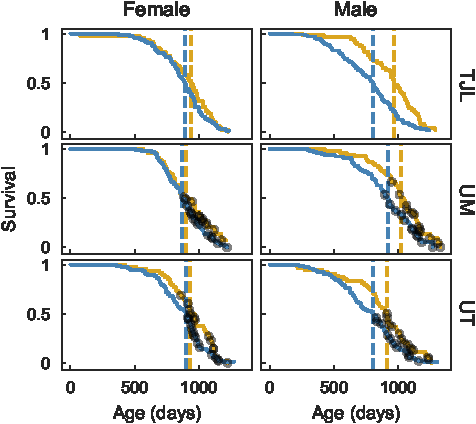
\includegraphics{fig/survival_sample.pdf}
  \caption{\label{fig:survival_sample}\csentence{Survival curves of sampled cohort.}
  Survival curves for mice fed a control diet (blue lines) or mice fed the same
  diet containing ACA (gold) at each of three sites: TJL, UM, and UT\@.
  Median longevity for each group of mice is indicated by a dashed vertical line.
  Black circles indicate the age at death for each of the sampled mice at UM and
  UT\@.
  }
\end{figure}

\subsection*{Differences in fecal community in ACA-treated mice}

ACA-treated mice had a substantially different microbial community composition
from control mice at all three study sites.
In a multivariate analysis of variance on site, sex, and treatment
using Bray-Curtis dissimilarities and including
all two-way interactions, significant effects were found for treatment
($\mathrm{partial} \; r^{2} = 9.6\%$, PERMANOVA $P < 0.001$)
and site ($\mathrm{partial} \; r^{2} = 16.4\%$, $P < 0.001$),
as well as their interaction ($\mathrm{partial} \; r^{2} = 3.4\%$, $P < 0.001$).
These statistical results reflect the separation apparent in a
principal coordinates ordination (see Fig.~\ref{fig:comm_pcoa}).
A much smaller but still significant effect of sex
($\mathrm{partial} \; r^{2} = 1.0\%$, $P = 0.014$) was also identified,
but there was no interaction between sex and treatment ($P = 0.344$).
Despite the unbalanced design, significance of the PERMANOVA was not affected
by changing the order of predictors.
Based on a test of multivariate homogeneity of variances,
dispersion differed between sites (PERMDISP $P < 0.001$)
and sexes ($P = 0.023$), which may bias the PERMANOVA results,
but did not differ between treatments ($P = 0.425$).
The small effect of sex and the lack of significant interaction effects with
treatment suggest that community composition itself, at the level of overall
diversity, is not directly
responsible for differential effects of ACA on longevity in male and female
mice.
However, the substantial differences in community composition due to treatment,
while not surprising, suggests that the effects of ACA on the microbiome have
the potential to modulate host health.

\begin{figure}[h!]
  \includegraphics{fig/comm_pcoa.pdf}
  \caption{\label{fig:comm_pcoa}\csentence{Microbial community composition.}
  Fecal bacterial community composition in mice fed the control diet (circles)
  or the same diet supplemented with ACA (triangles).
  The two dominant principal coordinates, based on Bray-Curtis dissimilarities
  among community profiles, are plotted, and percent of
  variation explained by each is indicated in parentheses on the axes.
  The location of points in each panel is identical.
  Markers denote whether mice were treated (triangles) or controls
  (circles).
  In (\textbf{A}) points are colored by treatment: control mice (blue)
  and ACA-treated (gold), in
  (\textbf{B}) points are colored by site: TJL (pink), UM (blue), and UT (green),
  and in (\textbf{C}) points are colored by sex: male (light blue) and female (pink).
  }
\end{figure}

The fecal bacterial community in control mice was dominated by a handful
of bacterial families (see Tbl.~\ref{tbl:aca_family} for details).
Across control mice at all three sites, a median of 30\% of sequences were
classified as members of the largely uncultured family
\taxon{Muribaculaceae}---historically called the S24-7---belonging to the
phylum Bacteroidetes.
Other abundant families included the Lachnospiraceae (27\%),
Ruminococcaceae (14\%), Lactobacillaceae (9\%), and Erysipelotrichaceae (1\%),
all of which are classified in the phylum Firmicutes.
More than 99.99\% of sequences across all mice were classified at or below the
family level.
More detailed classification of sequences is provided in an additional file
(see Appendix~\ref{app:otu_details_table}).

At a 97\% sequence similarity cutoff, 271 operational taxonomic units (OTUs)
had a mean relative abundance across all samples of greater than 0.01\% and an
incidence of greater than 5\%.
Of these, the relative abundance of 113 OTUs differed between treated
and control mice, correcting for a false discovery rate (FDR) of 5\%.
Together, these OTUs account for a median relative abundance of 54\% across
both control and treated mice.
OTUs differing between sexes or reflecting an interaction between sex and
treatment were a substantially less abundant.
5 OTUs were identified after FDR correction that differed
significantly in relative abundance between male and female mice,
accounting for a median, summed relative abundance of 6\%.
7 OTUs were found to be subject to an interaction between treatment and
sex, with a median relative abundances of 2\%.
Details of OTUs responsive to treatment, sex,
and a treatment-by-sex interaction have been included in an additional file
(see Appendix~\ref{app:otu_details_table}).

Differences between control and ACA mice at TJL and UM were dominated by
the increased abundance of a single OTU, OTU-1,
which had a median relative abundance of 7.7\% in control mice
compared to 28.8\% in ACA mice at TJL (Mann-Whitney U test $P < 0.001$),
and 10.4\% compared to 39.0\% at UM ($P < 0.001$) (see
Fig.~\ref{fig:dominant_otus_box}).
At UT, OTU-1 was higher in ACA-treated mice---a median of 5.4\% and 11.0\% in
control and treated mice, respectively---but this increase was not
statistically significant ($P = 0.344$).
Instead, a different OTU, designated OTU-4,
was strongly affected by ACA treatment at UT,
with a median relative abundance of 6.3\% in control mice
that increased to 25.6\% in ACA-treated mice ($P = 0.007$).
OTU-4 was nearly absent at TJL and UM, with only one mouse out of 95
having a relative abundance above 0.1\%,
compared to 39 out of 48 mice at UT\@.
Differences in abundance between sexes were not observed for OTU-1 at TJL or
UM, but at UT results were suggestive of an increased abundance of OTU-1 in
females ($P = 0.076$) and an increased abundance of OTU-4 in males ($P = 0.060$).
Interestingly, their combined abundance did not differ between males and
females ($P = 0.344$) at UT\@.
Both OTU-1 and OTU-4 were classified as members of the \taxon{Muribaculaceae}, and
subsequent phylogenetic analysis confirmed this placement (Appendix~\ref{app:otu_tax}).
OTU-1 and OTU-4 are approximately 90\% identical
to each other and to the most closely related cultivar (DSM-28989)
over the V4 hypervariable region of the 16S rRNA gene.
These OTUs are notable both for their high abundance overall,
as well as the large difference between control and ACA-treated mice.
It is surprising that OTU-4 is common and differentially abundant at UT, while
remaining rare at both of the other sites, suggesting that local community
composition modulates the effects of ACA\@.
While OTU-1 is made up of multiple unique sequences, the composition within the
OTU does not differ substantially with ACA treatment
(see Fig.~\ref{fig:s247_phylotypes}).

\begin{figure}[h!]
  \includegraphics{fig/dominant_otus_box.pdf}
  \caption{\label{fig:dominant_otus_box}\csentence{Abundance of dominant OTUs.}
  Relative abundance of the 16S rRNA gene from two OTUs abundant in ACA-treated
  mice.
  Points in each panel correspond with samples collected from individual mice at
  each of three replicate study sites.
  Samples were obtained from mice fed either the control diet
  (blue)
  or the same diet supplemented with ACA (gold).
  Markers indicate the sex of the mouse: male (triangle) or female (circle).
  Boxes span the interquartile range and the internal line indicates the
  median.
  (*: $P < 0.05$, **: $P < 0.001$ by Mann-Whitney U test).
  }
\end{figure}

The increased relative abundance of OTU-1 and OTU-4 in mice treated with
ACA appears to be due to greater abundance of these sequences, and is not
explained solely by a decrease in other groups.
The abundance of taxa in control and treated mice was
compared based on the recovery of spiked-in standard relative to the sequence
of interest.
The median combined spike-adjusted abundance of 16S rRNA gene copies from OTU-1
and OTU-4 was 4.3 times greater per gram of feces in ACA-treated mice compared
to controls (Mann-Whitney U test $P < 0.001$),
suggesting a corresponding increase in population density.

\begin{figure}
\includegraphics{fig/s247_phylotypes.pdf}
  \caption{\label{fig:s247_phylotypes}\csentence{Relative abundance across samples of unique sequences.}
  Distribution of common unique sequences clustered
  into (\textbf{A}) OTU-1 and (\textbf{B}) OTU-4.
  Colors are assigned to the top four most common unique sequences within each
  OTU and all remaining sequences from that OTU are assigned the color gray.
  Stacked bars in each position represent individual mice sampled for this study,
  and reflect the relative abundance of unique sequences in that sample.
  Mice are grouped into sites and then treatments, and finally by the
  total abundance of OTU-1.}
\end{figure}

While OTU-1 and OTU-4 are classified to the same family and are similarly
affected by ACA, other OTUs in the \taxon{Muribaculaceae} have decreased abundance in
treated mice.
The combined relative abundance of
all other OTUs in the family---excluding OTU-1 and OTU-4---was
8.3\% in treated mice versus 16.8\% of sequences in control mice
(Mann-Whitney U test $P < 0.001$).
The median combined spike-adjusted abundance of all other \taxon{Muribaculaceae} OTUs
was 0.5 times the median in control mice ($P = 0.001$), suggesting a
decrease in the population density of these taxa.
This is consistent with competition between OTUs in this family.

Three of the five most abundant families all exhibit decreased relative
abundance in ACA treated mice (see Tbl.~\ref{tbl:aca_family}).
However, the large increase in abundance of OTU-1 and OTU-4
suggests that some changes in the relative abundance of other taxa may be the
result of compositional effects, rather than decreased density.
For instance, although the relative abundance of Ruminococcaceae was lower in
ACA-treated mice, the spike-adjusted abundance was little changed ($P = 0.327$),
emphasizing the value of this complementary analysis.
Conversely, decreased relative abundance was matched by decreased
spike-adjusted abundance for both the Lactobacillaceae ($P = 0.014$) and
the Erysipelotrichaceae ($P = 0.063$).

\begin{table}[h]
\caption{\label{tbl:aca_family}Abundance of common bacterial families.}
  \begin{tabular}{rlll}
    \hline
    family                      & \% control\textsuperscript{a}  & \% ACA\textsuperscript{a}              & ACA : control\textsuperscript{b} \\
    \hline
    \taxon{Muribaculaceae}      & 30.4 (21.5, 43.3)              & 48.1\textsuperscript{**} (35.3, 61.8) & 1.8\textsuperscript{**} \\
    \taxon{Lachnospiraceae}     & 26.6 (16.3, 41.6)              & 23.9\textsuperscript{†}  (9.6, 37.4)  & 1.3 \\
    \taxon{Ruminococcaceae}     & 14.2 (9.0, 19.0)               & 11.6\textsuperscript{*}  (6.9, 15.6)  & 1.1 \\
    \taxon{Lactobacillaceae}    & 9.5  (1.2, 17.0)               & 2.6\textsuperscript{*}   (1.0, 8.2)   & 0.31\textsuperscript{*} \\
    \taxon{Erysipelotrichaceae} & 1.4  (0.3, 6.2)                & 0.5\textsuperscript{*}   (0.2, 2.2)   & 0.42\textsuperscript{†} \\
    \hline
  \end{tabular}
  \vspace{2mm}
  \begin{flushleft}
  \textsuperscript{a} Median and interquartile range of the relative abundance of the
  top five most abundant bacterial families in control and ACA-treated mice \\
  \textsuperscript{b} the ratio of median spike-adjusted abundances in ACA-treated mice versus control mice \\
  \textsuperscript{†}  $P < 0.1$   via Mann Whitney U test \\
  \textsuperscript{*}  $P < 0.05$  \\
  \textsuperscript{**} $P < 0.001$ \\
  \end{flushleft}
\end{table}



ACA-treated mice exhibited decreased fecal community diversity.
The median Chao1 richness estimate was decreased from
229 in control mice to 199 in treated mice
(Mann-Whitney U test $P < 0.001$).
The Simpson's evenness index was also lower in ACA mice:
0.044 versus 0.075 in controls ($P < 0.001$).
This reduced richness and evenness is not surprising given the much greater
abundance of a single OTU in treated mice at each site.
To understand changes in diversity while controlling for compositional effects,
we measured the effect of ACA ignoring counts for OTU-1 and OTU-4.
While Simpson's evenness was not decreased by treatment in this fraction of
the community ($P = 0.26$), the Chao1 richness---subsampling to equal counts
\emph{after} partitioning---was ($P = 0.005$),
suggesting that the bloom of OTU-1 and OTU-4 may have, in fact, resulted in the
local extinction of rare community members.

\subsection*{Changes in fecal metabolite concentrations}

Long-term ACA treatment affects metabolite profiles, increasing
concentrations of the SCFAs in feces (see Fig.~\ref{fig:scfa_box}).
Butyrate concentrations were increased
from a median of 3.0 mmols/kg wet weight in control mice to 4.9 in ACA-treated
mice (Mann-Whitney U test $P < 0.001$).
Propionate concentrations were also increased: a median of 1.1 in controls
compared to 2.3 with ACA ($P < 0.001$).
Median acetate concentrations were higher, 16.2 mmols/kg versus 12.9 in
controls, but a Mann-Whitney U test did not surpass the traditional
p-value threshold ($P = 0.073$).
The summed concentrations of acetate, butyrate, and propionate
was greater in ACA-treated mice, with a median concentration of 25.4 mmols/kg
versus 19.0 mmols/kg in control mice ($P = 0.003$).
This confirms our predictions given the expectation of greater
availability of polysaccharide substrate for fermentation.
Indeed, median glucose concentration was also increased from 5.3 to 10.3
($P < 0.001$).
Concentrations of formate, valerate, isobutyrate, and isovalerate
were generally below the detection limit.
Fresh pellet weight was increased from a median of 36 to 74 mg ($P < 0.001$)
Fecal starch content was not measured,
but pellets from ACA-treated mice had a noticeably chalky appearance.

\begin{figure}[h!]
  \includegraphics{fig/scfa_box.pdf}
  \caption{\label{fig:scfa_box}\csentence{Fecal metabolites.}
  Concentrations of metabolites in feces obtained from mice fed either the
  control diet (blue)
  or the same diet supplemented with ACA (gold).
  Boxes span the interquartile range and the internal line indicates the
  median.
  The shaded region highlights the three major SCFAs produced by
  microbial fermentation of polysaccharides in the gut, and the sum of their
  concentrations is plotted as ``total SCFA''.
  Above 0.1 mmols/g, concentrations are plotted logarithmically.
  (†: $P < 0.1$, *: $P < 0.05$,
  **: $P < 0.001$ by Mann-Whitney U test).
  }
\end{figure}

Butyrate as a molar percentage of total SCFA was modestly greater in the ACA
mice, a median of 19\% in control mice was increased to 22\% in treated mice
(Mann-Whitney U test $P < 0.001$),
as was propionate: 7\% in control, 10\% in treated ($P = 0.006$),
while acetate was decreased
from 73\% in controls to 66\% in treated mice ($P < 0.001$).

In contrast to the three measured SCFAs and glucose,
both succinate and lactate concentrations were decreased.
Median lactate was decreased from 3.2 mmols/kg in control mice to 1.3 in
ACA-treated mice ($P = 0.003$),
and succinate from 3.0 to 1.6 ($P < 0.001$).
It is surprising that these fermentation intermediates are reduced, given
the expected increase in available polysaccharide.
It is possible that their concentrations reflect greater consumption
in downstream pathways, or
perhaps ACA directly inhibits the metabolism and growth of relevant bacteria;
such effects have been previously reported for \frnlang{in vitro} fermentations of
starch with human fecal slurries~\cite{Weaver1997}.

Differences in SCFAs between sexes are particularly interesting given
the greater longevity effects of ACA in male mice.
For propionate, a sex-by-treatment interaction was found (ANOVA $P = 0.023$),
but butyrate and acetate had no such effect.
This interaction results in a larger difference in propionate concentrations
for male mice (from 1.4 mmols/kg in control to 2.7 in ACA) than for female mice
(from 1.0 to 1.9) with ACA treatment.
The significance of the interaction term was not corrected for
multiple testing, and therefore additional studies would greatly increase our
confidence in this result.
Fecal metabolite concentrations also varied over study site and sex of the
mouse;
effects of ACA stratified by site and sex are visualized in Fig.~\ref{fig:stratified_metab}.

\subsection*{Community predictors of fecal SCFA concentrations}

Community composition was correlated with metabolite concentrations
in both control and ACA-treated mice.
Numerous strong correlations were detected between the
spike-adjusted abundance of 16S rRNA copies from the most common bacterial
families and the concentrations of SCFAs and lactate.
Notably,
\taxon{Muribaculaceae} abundance was particularly strongly correlated with
propionate concentrations in both control
(Spearman's $\rho = 0.36$, $P = 0.002$; see Fig.~\ref{fig:metab_corr})
and ACA mice ($\rho = 0.64$, $P < 0.001$).
Likewise, Lachnospiraceae were correlated with butyrate ($\rho = 0.61$ in control
and $0.77$ in ACA, $P < 0.001$ for both),
and Lactobacillaceae with lactate concentrations ($\rho = 0.63$ in control
and $0.67$ in ACA, $P < 0.001$ for both).
Strikingly, concentrations of acetate and butyrate were especially correlated
with each other
($\rho = 0.67$ in control and $0.80$ in ACA, $P < 0.001$ for both).
Although our study was not an unambiguous test, these results
support the hypothesis that the fecal metabolite response to treatment is
dependent on the population density of relevant microbes in the gut community.
Similarly, environmental and host factors that promote or inhibit the growth
of particular community members would be expected to modulate the response.

\begin{figure}[h!]
  \includegraphics{fig/metab_corr.pdf}
  \caption{\label{fig:metab_corr}\csentence{Microbiota/metabolite correlations.}
  Correlations among metabolite concentrations in feces and family level,
  spike-adjusted 16S rRNA gene abundances.
  Points correspond with samples collected from individual mice and colors
  indicate whether they were obtained from mice fed the control diet
  (blue)
  or the same diet supplemented with ACA (gold).
  Markers indicate the sex of the mouse: male (triangle) or female (circle).
  Metabolite concentrations are reported normalized to feces wet weight, and
  abundances are in spike-equivalent units.
  Values are on a linear scale between 0 and the
  subsequent tick label, above which, points are plotted logarithmically.
  }
\end{figure}

To identify key players in these associations,
we examined the relationship between metabolite concentrations and the
spike-adjusted abundances of OTUs.
Based on a LASSO regression, the abundances of a number of OTUs can be used to
predict concentrations of
propionate, butyrate, acetate, and lactate even after accounting for treatment,
sex, and study site.
Consistent with the correlations found between \taxon{Muribaculaceae} abundance and
propionate, OTU-1 and OTU-4 were identified as predictors of increased
propionate, along with a third taxon, OTU-5, also classified as a member of the
family.
For both butyrate and acetate,
OTUs classified as members of both the Lachnospiraceae
and Ruminococcaceae were most predictive of increased concentrations.
Unsurprisingly, the most abundant OTU classified as a member of the
Lactobacillaceae, OTU-2, was found to be highly predictive of increased
lactate.
However, 8 OTUs were also associated with decreased lactate
concentrations, most of which were among those associated with increased
butyrate and acetate.
Among other explanations, this is consistent with these taxa either being
inhibited by lactate or being lactate utilizers, which are likely to be
producing SCFAs as secondary fermentation products.
Regression coefficients
for each metabolite are included in an additional file (see Appendix~\ref{app:otu_details_table}).
Overall, results were both consistent with \frnlang{a priori} expectations, and
useful for generating hypotheses about which taxa might be associated with the
generation of fermentation products.

\subsection*{Fecal SCFA concentrations as predictors of longevity}

Given the documented health benefits of SCFAs in the gut (reviewed in~\cite{Koh2016})
and their increased levels in ACA-treated mice, we tested the relationship
between the acetate, butyrate, and propionate concentrations in feces,
and the lifespan of individual mice.
Lifespans of fecal donors were not available for mice at TJL,
so survival analyses were carried out only with UM and UT mice,
and effect sizes are reported for SCFAs as standardized hazard
ratios (HRs).
Due to the reduced number of mice sampled for this study, data were pooled
across sexes and sites.
The shared effects of the
design parameters---treatment, sex, and study site---on both SCFAs
and longevity, were accounted for by including terms for these covariates as
well as their two and three-way interactions.
Analyses reinforcing our interpretations are discussed in Appendix~\ref{app:expand_surv}.
Tested individually against this null model, an association between longevity
and propionate was found (standardized HR of 0.727, $P = 0.031$), but no
relationship was found with butyrate ($P = 0.240$) or acetate ($P = 0.742$).
However, when the model was fit with all three SCFAs simultaneously,
each was found to be associated with longevity
($P = 0.012$, $0.030$, $0.042$ for propionate, butyrate, and acetate, respectively).
Coefficients for SCFA covariates in this full model suggest a positive
association with longevity for both propionate and butyrate
(standardized HR of 0.674 and 0.586, respectively).
Interestingly, a negative association was found with
acetate (standardized HR of 1.576) using this model.
The discrepancy between this result and the lack of association when butyrate
and acetate are each tested alone likely reflects the strong positive
correlation between acetate and butyrate concentrations, masking their
individual, opposing associations with longevity.
The overall fit of the full model was improved
compared to the null model with only design covariates
(likelihood ratio test, $P = 0.023$).

\section*{Discussion}

ACA, by inhibiting the enzymes responsible for starch degradation in the small
intestine, is expected to increase the availability of this polysaccharide to
the microbiome.
The resulting increase in SCFA production may contribute to the effects of ACA
on health.
Despite previous observations in humans and rats that ACA results in
substantial changes to the community structure~\cite{Zhang2017, Weaver1997} and
fermentation products~\cite{Dehghan-Kooshkghazi2004, Weaver1997, Weaver2000, Wolin1999} of the gut
microbiota, a link between these effects on the microbiome and longevity has
not been established.
Here we present the first study to combine
bacterial community surveys with measurement of fecal metabolites in ACA
treated mice, as well as the first to pair these data with lifespan,
allowing us to explore the role of the microbiome in increased longevity.

Our results confirm all four predictions that we set out to test:
ACA was found to affect both (1) the composition of bacterial communities and
(2) SCFAs in mouse feces,
(3) the abundances of individual taxonomic groups were associated with
concentrations of fermentation products,
and (4) the concentrations of fecal SCFAs were associated with variation in
mouse longevity.

While it is unsurprising that an increased flux of starch to the large
intestine affected the gut microbiota and their fermentation products,
some changes were especially pronounced.
The increased relative abundance in ACA-treated mice of the dominant
OTU---OTU-1 at UM and TJL and OTU-4 at UT---was
dramatic:
one or the other was increased approximately 4-fold at all three sites
and in multiple samples more than half of sequences belonged to these OTUs.
A cursory BLAST search reveals that sequences identical to OTU-1 have been
previously recovered in published studies (e.g.~\cite{Lowe2017} and~\cite{Castoldi2017});
in \cite{Singer2017} the sequence was found at high relative
abundance in the brains of mice that had undergone sepsis.
It was notable that OTU-1 did not respond to ACA at UT, while its increased
abundance was so striking at UM and TJL\@.
Our results appear to constrain the potential explanations for this
observation.
OTU-1 was present and abundant at all three sites;
The abundance in control mice was lowest at UT, although the median there was
still greater than 5\%.
While it is not possible with the data presented here to rule out genomic
differences of OTU-1 among sites, a similar composition of unique
16S rRNA gene sequences made up this cluster at all three.
On the other hand, OTU-4 was at very low abundance, with no reads in a majority
of samples, at UM and TJL where OTU-1 did respond to ACA\@.
These results suggest that both OTUs respond to ACA in the same way,
with OTU-4, when it is sufficiently abundant, inhibiting the response of OTU-1,
potentially through resource competition.
Both OTUs are in the same family, the \taxon{Muribaculaceae}, but are not the same
species or genus by the traditional similarity thresholds, sharing only 90\%
identity over the sequenced fragment.
The differential response of these OTUs among sites illustrates the
importance of each site's local ``metacommunity'' in determining the microbial
community's response to environmental perturbations.

Pronounced differences in the resident microbial communities of different hosts
may contribute to challenges in translating results from mice and other model
organisms to humans.
A comparison of bacterial community composition in feces in prediabetic
people before and during a 4-week ACA treatment period did
not reveal changes of the magnitude reported here~\cite{Zhang2017}, although this may reflect
the limited duration of treatment.
Interestingly, in that study \taxon{Lactobacillaceae} abundance increased with ACA,
while we observed this family to be depleted in treated mice.
The abundance of the \taxon{Muribaculaceae} was not reported.
Although this family is common in mice
and have been previously shown to respond to diet,
the clade is substantially less abundant in most human samples~\cite{Ormerod2016}.
However, the prevalence of \taxon{Muribaculaceae} may be under-reported in the
literature, as the Ribosomal Database Project~\cite{Cole2014} does not include the
family and classification using this database assigns sequences to the
\taxon{Porphyromonadaceae} instead~\cite{Clavel2016}.
Historically, two other names have also been used for this clade: the ``S24-7''
(from an early environmental clone~\cite{Salzman2002}),
and ``\taxon{Candidatus Homeothermaceae}'' (proposed in~\cite{Ormerod2016}).
While the isolation of one \taxon{Muribaculaceae} cultivar has recently been
published, \taxon{Muribaculum intestinale} YL27~\cite{Lagkouvardos2016},
and as of this writing several draft genomes are available for unpublished
isolates (e.g.~see whole genome shotgun sequencing projects NWBJ00000000.1 and
NZ\_NFIX00000000.1),
additional cultivars will be vital for understanding the function and ecology
of the family.
Nonetheless, genomes assembled from metagenomes suggest that populations of
\taxon{Muribaculaceae} are equipped with fermentation pathways to produce succinate,
acetate, and propionate, and that the family is composed of metabolic guilds,
each specializing on the degradation of particular types of polysaccharides:
plant glycans, host glycans, and $\alpha$-glucans~\cite{Ormerod2016}.
This suggests that the \taxon{Muribaculaceae} may occupy a similar set of niches in
mice as do \taxon{Bacteroides} species in humans.
The \taxon{Muribaculaceae} and \taxon{Bacteroides} are both in the order
\taxon{Bacteroidales}.
\taxon{Bacteroides} also specialize in the fermentation of
polysaccharides~\cite{Wexler2007}, and at least some of the most common species in the human gut
are known to produce succinate, acetate, and propionate from the fermentation
of polysaccharides~\cite{Song2015, Macy1978, Macfarlane2003, Koh2016}.
Unlike the patterns observed here for \taxon{Muribaculaceae} in mice,
the abundance of \taxon{Bacteroides} decreased with ACA treatment in
one study in humans~\cite{Zhang2017}, suggesting that the microbially mediated
effects of ACA may fundamentally differ between these hosts.

Besides hypotheses based on genome content,
the correlation between total \taxon{Muribaculaceae} abundance and propionate
concentrations and the specific association with OTU-1 and OTU-4
found in the LASSO analysis
suggest that both OTUs, and perhaps other
\taxon{Muribaculaceae} species in this study, ferment starch to propionate.
This also supports the hypothesis, discussed above, that both OTUs occupy
overlapping niches.
Although increased butyrate concentrations have been frequently reported with
ACA treatment~\cite{Weaver1997, Wolever2000, Dehghan-Kooshkghazi2004, Weaver2000, Wolin1999},
elevated concentrations of propionate have been observed in
just one previous study using portal blood in rats~\cite{Dehghan-Kooshkghazi2004}.
Studies in humans have instead found decreased
or no change in fecal~\cite{Holt1996, Weaver1997, Weaver2000} or
serum~\cite{Wolever2000} propionate concentrations with ACA\@.
Decreased propionate has been
attributed to preferential production of butyrate from starch
fermentation~\cite{Weaver1992, Cummings1987} or inhibition of propiogenic
bacteria by ACA~\cite{Weaver1997}.
Our observation of increased propionate was robust and reproduced at all three
sites.
If this conflicting result reflects both the greater initial abundance and
enrichment in our study of the \taxon{Muribaculaceae}---especially OTU-1 and
OTU-4--- it demonstrates the value of measuring both community composition
and metabolite concentrations in the same samples.

SCFAs are commonly suggested to act as intermediaries between the gut
microbiota and host physiology~\cite{Koh2016}.
While our study was not designed to provide a causal test of effects of
SCFAs on longevity, and the power of our analysis was limited,
a statistical association between
SCFA concentrations and mouse lifespan supports an interpretation
that is consistent with an extensive literature on the health benefits of
butyrate and propionate~\cite{Koh2016}.
In addition, that SCFA concentrations were associated with longevity above and
beyond the effects of ACA, study site, and sex, further supports this
hypothesis.
It is somewhat surprising, however, that a single fecal sample taken, in some
cases, several months before death, could be predictive of longevity.
The association reported here could reflect other, unmeasured, changes in the
gut microbiome or host physiology.
Concentrations of metabolites in feces are an integration of both
production and consumption rates along the length of the lower gut, and may not
reflect host exposure nor the strength of host physiological response.
It is also important to note that, since all mice in this study at the time of
sampling were of an age close to the median lifespan of control individuals,
the results are only relevant to mechanisms of aging in late-life and should
not be extrapolated to young mice.
Experimental tests of a causal role for SCFAs in longevity will be challenging,
as they likely require controlled manipulation of intestinal SCFAs for the
lifetime of a mouse.

Due to the preferential enhancement of longevity by ACA in male mice we sought
to identify aspects of the gut microbiome that responded differently in male
and female mice (i.e.~interaction effects), as these might suggest mechanistic
explanations for differences in longevity effects~\cite{Harrison2014}.
While we do not believe that the magnitude of sex-by-treatment interactions
observed for various aspects of the microbiome were sufficiently pronounced to
fully explain the differential effect of ACA on lifespan, our search was
limited by sample size, variability between study sites, and the large number
of features being tested.
Nonetheless, ACA was found to increase propionate concentrations more in male
mice than females, a statistically significant pattern before correction for
multiple testing, and the relative abundance of a handful of OTUs seem to have
also been subject to an interaction.

Mechanisms unrelated to the gut microbiome have been proposed for the effects
of ACA on lifespan.
Because ACA reduces the postprandial glucose spike observed in mice and humans,
hypotheses emphasizing the reduction of harmful effects associated with these
transient surges have been most commonly invoked.
Studies of UM-HET3 mice given ACA from 4 to 9 months of age suggested that
mean daily blood glucose levels are minimally affected, but that absorption of
glucose was both slower and longer lasting~\cite{Harrison2014}.
Interestingly, fasting insulin level in ACA-treated males are much lower than
those in control males, consistent with an improvement in insulin
sensitivity~\cite{Harrison2014}.
This reduction was not seen in females, where insulin levels in controls were
lower than in control males and similar to those in ACA-treated
males~\cite{Miller2014, Harrison2014}, presenting one possible explanation for the
stronger longevity benefit in males.
Still, the connection between this modulation of postprandial
glucose---with or without improved insulin sensitivity---and extended
longevity is still far from certain.

The work presented here explores a different hypothesis:
that health benefits in ACA mice are related to changes in the activity
of microbial communities in the gut associated with the increased influx
of starch, and possibly attributable to known health effects of microbial
metabolites, including SCFAs.
The changes described here in both community composition and fermentation
products due to ACA treatment, along with the statistical association between
fecal SCFA concentrations and longevity, are consistent with this hypothesis,
and provide a stepping-stone for future studies.
Interestingly, SCFAs themselves have well documented effects on glucose
homeostasis (reviewed in~\cite{Morrison2016} and~\cite{Canfora2015}).
The two explanations are therefore not mutually exclusive, and
the effects of ACA on longevity may be mediated by both
glucose physiology and microbial activity in the gut.

\section*{Conclusions}

Here we have tested four predictions of a proposed model connecting
ACA to lifespan via the gut microbiome.
We demonstrate that ACA reproducibly modulates the composition
of the microbiota, as well as the concentrations of fermentation products,
increasing the abundance of butyrate and propionate.
In addition, we provide evidence that the structure of the microbial
community is an important factor in the composition of metabolites produced.
Finally, we show an association between SCFA concentrations in feces and
survival, suggesting a role of the microbiome in the life-extending properties
of ACA\@.
Together, these results encourage a new focus on managing the gut microbiota
for host health and longevity.

\section*{Methods}

\subsection*{Mouse housing and ACA treatment}

Mice were bred and housed, and lifespan was assessed as described in~\cite{Harrison2014}.
Briefly, at each of the three study sites, genetically heterogeneous, UM-HET3,
mice were produced by a four-way cross as previously described in~\cite{Miller2011}.
After weaning, mice were fed LabDiet\textsuperscript{\textregistered}~(TestDiet Inc.)
5LG6 produced in
common batches for all sites.
At 42 days of age, electronic ID chips were surgically implanted and treatment
randomly assigned to each cage housing four mice to a cage for females
and three to a cage for males.
ACA-treated mice were fed the same chow amended with 1000 ppm ACA
(Spectrum Chemical Manufacturing Corporation) from 8 months of age onwards.
Mice were transferred every 14 days to fresh, ventilated cages with
water provided in bottles.
Colonies at all three sites were assessed for infectious agents four
times each year, and all tests were negative for the entire duration of the
study.

\subsection*{Sample collection and processing}

Fresh fecal pellets were collected directly from mice between 762 and 973 days
of age and frozen at -80°C.
We did not control the time of day at collection.
While differences in age and collection time could have added variability to
SCFA concentrations, both were similarly distributed for the different
treatment groups, so they are unlikely to confounded our analyses.
To eliminate potential cage effects from co-housed mice~\cite{Laukens2015},
samples were obtained from no more than one randomly selected mouse per cage.
A total of 144 samples were collected from 12 male and 12 female mice in both
control and ACA treatment groups at each of the three sites.
Samples were shipped on dry ice and then stored, frozen, until processing.
For approximately the first half of samples, we extracted the soluble fraction
by homogenizing pellets with 200~$\mu$L of nuclease-free water.
For the remaining samples, we instead used a 1:10 ratio (weight:volume), with a
maximum volume of 1.5~ml.
This was found to improve quantification in higher weight samples.
While SCFA concentration estimates were higher when using the amended protocol,
the order of sample extraction was fully randomized, so it is unlikely to have
biased our interpretations.
Homogenized samples were centrifuged at 10,000~×~g for 10~minutes to
separate soluble and solid fractions.
The supernatant was then serially vacuum filtered, ultimately through a
0.22~$\mu$m filter, before HPLC analysis.
The solid fraction was frozen prior to DNA extraction.
Four samples were excluded from chemical analysis and one from DNA analysis due
to technical irregularities during sample processing.

Prior to DNA extraction, fecal pellet solids were thawed and, where
necessary, subsampled for separate analysis.
To move beyond relative abundance, solids were weighed and
spiked with 10~$\mu$L aliquots of prepared \taxon{Sphingopyxis~alaskensis} strain
RB2256---an organism not found in mouse feces---in order to compare
16S rRNA gene abundance between samples~\cite{Smets2016, Stammler2016}.
The spike was prepared as follows:
a 1:200 dilution of a stationary phase \taxon{S.~alaskensis} culture was grown at
room temperature for approximately 44 hours in R2B medium with shaking.
This culture was harvested at a final OD420 of 0.72 before being rinsed in PBS
and resuspended---5-fold more concentrated---in 20\% glycerol in
PBS (v/v).
Aliquots of these cells were stored at -20°C before extraction and
sequencing.
Spiked fecal samples were homogenized in nuclease free water at a ratio of
1:10 (w/v).
DNA was extracted from 150~$\mu$L of this mixture using the MoBio PowerMag
Microbiome kit.

\subsection*{Chemical analysis}

The chemical composition of samples was assessed
on a Shimadzu HPLC (Shimadzu Scientific Instruments) equipped
with an RID-10A refractive index detector.
30~$\mu$L injections were run on an Aminex HPX-87H column
(Bio-Rad Laboratories, Hercules, CA) at 50°C with 0.01~N H\textsubscript{2}SO\textsubscript{4} mobile
phase and a flow rate of 0.6~ml/minute.
External standards were run approximately daily containing
acetate, butyrate, formate, glucose, lactate, propionate, and succinate
at 8 concentrations between 0.1~mM to 20~mM.
Due to the complexity of the chromatogram, the identity
and area of retained peaks was curated manually,
assisted by the LC Solutions Software (Shimadzu Scientific Instruments)
Standard curves were fit using weighted regression (inverse square of the
concentration), and, for all compounds except propionate,
without an intercept.

\subsection*{16S rRNA gene sequencing and analysis}

The V4 hypervariable region of the 16S rRNA gene was amplified from extracted
DNA (as described in~\cite{Kozich2013}), and sequenced on an Illumina MiSeq
platform using a MiSeq Reagent Kit V2 500 cycles (cat\# MS-102-2003).
Amplicon sequences were processed with MOTHUR (version~1.39.4~\cite{Schloss2009})
using a protocol based on the 16S standard operating procedures~\cite{Kozich2013}.
Scripts to reproduce our analysis can be found at
\url{https://github.com/bsmith89/smith2018paper}.
After fusing paired reads, quality trimming, and alignment to the
SILVA reference database (Release~132 downloaded from~\cite{Schloss2018}).
The vast majority of 16S rRNA gene sequences were between 244 and 246 bp.
Sequences were classified using the method of Wang et al.~\cite{Wang2007} as
implemented in MOTHUR and with the SILVA non-redundant database as a
reference~\cite{Yilmaz2014}.
We clustered sequences into OTUs using the
OptiClust method~\cite{Westcott2017} at a 97\% similarity threshold.
We counted and removed sequences classified as \taxon{S.~alaskensis},
the spiked-in standard, before further analysis.
We did not attempt to assess the exact number of 16S rRNA gene copies spiked
into samples.
Instead, spike-adjusted abundance was defined in units based on
the standardized spike
($\mu\mathrm{L \; spike \; equivalents} \; / \; \mathrm{g \; sample}$)
and estimated using the formula:

\[
\mathrm{RelativeAbundance} \;\times\;
    \frac{(\mathrm{TotalEndemicReadCount} \;\times\; \mathrm{SpikeVolume})}
         {(\mathrm{TotalSpikeReadCount} \;\times\; \mathrm{SampleWeight})}
\]

Family level abundance was calculated as the summed abundance of all sequences
clustered in OTUs classified to that family.
OTU counts were randomly subsampled to the minimum number of reads before
calculating Chao1 richness, but were not subsampled for other analyses.
A single, independent realization of random subsampling was used for each
richness calculation.
A search of the NCBI non-redundant nucleotide database for
related sequences from cultured bacteria was carried out using the
BLASTn web tool~\cite{Wheeler2000} searching the non-redundant nucleotide database
with default parameters and excluding sequences from uncultured organisms.

\subsection*{Statistical analysis}

A 0.05 p-value threshold was used to define statistical significance, with
values below 0.1 considered ``suggestive''.
Except where specified, p-values are not corrected for multiple testing.
Due to the risk of violating distributional assumptions, univariate comparisons
between groups were done using the non-parametric Mann-Whitney U test.
Differences in multivariate community composition and dispersion were tested
using PERMANOVA (\compcmd{adonis}) and PERMDISP (\compcmd{betadisper}) respectively,
both implemented in the vegan package (version~2.4-6~\cite{Oksanen2018})
for the R programming language.
Bray-Curtis dissimilarity was used as the $\beta$-diversity index.

Differences in the relative abundance of individual OTUs were surveyed
using the DESeq2 package (version~1.18.1~\cite{Love2014a}) for R,
and fitting a model that included terms for treatment, sex, site, and
the interaction between treatment and sex.
So as to keep valuable distributional information,
all OTUs found in at least two samples were included in the initial analysis,
with p-values calculated using a Wald test.
However, FDR correction using the
Benjamini-Hochberg procedure~\cite{Benjamini1995} excluded ``rare'' OTUs---those
with mean relative abundance less than 0.01\% or detected in fewer than 5\% of
samples---in order to maintain statistical power by independently reducing
the number of tests.

Interactions between sex and treatment in fecal SCFAs were assessed for
log-transformed concentrations.
The small number of zeros were replaced with half the lowest detected
concentration for that metabolite.
Interactions were tested in an ANOVA that also included terms for site, sex,
and treatment.
LASSO regressions of the three SCFAs and lactate against spike-adjusted OTU
abundances were performed using the scikit-learn library for Python
(version~0.18.2~\cite{Pedregosa2012})
and log-transformed concentrations after adjustment
for site, sex, and treatment.
OTUs detected in more than 5\% of samples and with mean abundance greater
than 0.01\% were included.
The LASSO parameter was determined by randomized 10-fold cross-validation,
optimizing for out-of-bag R\textsuperscript{2}.
For each metabolite we confirmed that OTU abundance information improved
predictions by testing the Spearman's rank correlation
between true values and out-of-bag predictions of the best model using a
Student's t-distribution approximation~\cite{Iman1978} and a $P = 0.05$ significance
threshold.
While this type of regularized regression is primarily useful for constructing
predictive models, and biological interpretation can be challenging,
non-zero regression coefficients are suggestive of covariates that are among
the most strongly associated with a response.
Proportional hazards regression was carried out using of the
survival package (version~2.41-3~\cite{Therneau2015}) for R, and the day
of fecal sampling as the entry time.
All sampled mice were dead at the time of analysis and
right-censoring was therefore not used.
Standardized HRs reported for SCFAs are based on concentrations
that have been centered around 0 and scaled to a standard deviation of~1.


\FloatBarrier

\appendix

\section{Description of Additional file - OTU details table}\label{app:otu_details_table}

Summary statistics, associations with design parameters and metabolites, and
inferred taxonomic identity of common bacterial OTUs.
Table includes all OTUs with mean relative abundance greater than 0.01\% and
found in greater than 5\% of samples.
Associations with treatment, sex, and a treatment-by-sex interaction are
included in columns labeled ``treatment\_effect'', ``sex\_effect'', and
``interact\_effect'', respectively.
Columns labeled ``propionate'', ``butyrate'', and ``acetate'' include fitted
coefficients from the respective LASSO regression.
Formatting has been included to facilitate exploration, with background colors
indicating the sign and magnitude of coefficients and colored circles
indicating the statistical significance of results after FDR correction.

\section{Supplemental figure}\label{app:supp-figures}

\begin{figure}[h!]
\includegraphics{fig/scfa_box_supplement.pdf}
  \caption{\label{fig:stratified_metab}\csentence{Concentrations of metabolites stratified by site and sex.}
  Chemical analysis of feces obtained from mice fed either the
  control diet (blue)
  or the same diet supplemented with ACA (gold) within individual
  (\textbf{A}-\textbf{C}) study sites and (\textbf{D}-\textbf{E}) sexes.
  Markers indicate the sex of the mouse: male (triangle) or female (circle).
  Boxes span the interquartile range and the internal line indicates the
  median.
  The shaded region highlights the three major SCFAs produced by
  microbial fermentation of polysaccharides in the gut, and the sum of their
  concentrations is plotted as ``total SCFA''.
  Above 0.1 mmols/g, concentrations are plotted logarithmically.
  Significance symbols reflect differences in concentration between treated
  and control mice
  (†: $P < 0.1$, *: $P < 0.05$,
  **: $P < 0.001$ by Mann-Whitney U test).}
\end{figure}

\FloatBarrier

\section{Taxonomic analysis of two dominant OTUs}\label{app:otu_tax}

The most conspicuous difference in the gut microbiota induced by ACA was a
site-specific effect in two populations of bacteria both classified
as members of family \taxon{Muribaculaceae} (Fig.~\ref{fig:dominant_otus_box}).
OTUs were classified based on an approximately 240 bp fragment of the 16S rRNA
gene in the V4 hypervariable region.
Using this fragment, we applied several lines of evidence to confirm that OTU-1
and OTU-4 are both members of the \taxon{Muribaculaceae} and that they are
genetically distinct from cultured relatives.
Classification of sequences using the method of Wang et al. \cite{Wang2007} and the
SILVA non-redundant database as a reference \cite{Yilmaz2014}, identified both
OTU-1 and OTU-4 as members of the family with 100\% bootstrap support.
While use of the RDP training set \cite{Cole2014} Version 14 instead assigned
these sequences to the family Porphyromonadaceae
this is presumably because the \taxon{Muribaculaceae} are not recognized as a taxon
in the RDP (previously reported by \cite{Clavel2016}), nor are alternative names for
the clade (``S24-7'' or ``\taxon{Homeothermaceae}'').
A follow-up phylogenetic analysis of representative amplicon sequences from two
dominant OTUs was carried out using approximate maximum likelihood
estimation implemented in the FastTree software (version 2.1.8 \cite{Price2010}) using the
generalized time reversible model with twenty discrete rate categories
(\texttt{-gtr\ -gamma} options).
Approximate maximum likelihood phylogenetic estimation, using a selection of
type strains in the order Bacteroidales,
places OTU-1 and OTU-4 in a clade with representatives of the \taxon{Muribaculaceae}
with \textgreater{}95\% support for the topology of that node (see Fig.~\ref{fig:s247_tree}).
While such a short sequence fragment
is unlikely to perfectly recapitulate
phylogeny---indeed, tree topology was generally weakly supported
and was sensitive to both the choice of reference sequences
and the evolutionary model used---we are nonetheless satisfied with the
evidence for assignment of both OTU sequences to this clade;
besides exceptions in the Porphyromonadaceae, Marinilabiliaceae,
and \taxon{Bacteroides}, our phylogenetic reconstruction largely matches a recently
proposed taxonomy of the Bacteroidales \cite{Ormerod2016}.

\begin{figure}[h!]
  \includegraphics{fig/s247_tree.pdf}
  \caption{\label{fig:s247_tree}\csentence{Phylogenetic characterization of OTU-1 and OTU-4.}
  Estimated phylogeny based on approximately 240 bp of the 16S rRNA gene V4 hypervariable region
  and more than 130 type strain reference sequences spanning the diversity of
  order Bacteroidales.
  Branch lengths are in units of expected substitutions per site.
  The tree is rooted by a Flavobacteriales out-group (not shown).
  Reference taxa are labeled with genus designations according to the SILVA
  database.
  When multiple representatives from the same genus have been folded together,
  the number of sequences is reported in parentheses.
  Nodes with Shimodaira-Hasegawa local support over 95\% are indicated with black
  circles and nodes with support less than 70\% have been collapsed to polytomies.
  The dashed box encloses taxa inferred to be within the \taxon{Muribaculaceae}.
  The taxon labeled `S24-7 (clone)' (GenBank: AJ400263.1) is the environmental
  sequence by which the clade was originally identified, and by which it was
  historically named \cite{Salzman2002},
  while \taxon{Muribaculum intestinalis} (GenBank: KR364784.1) is the first
  cultured representative \cite{Lagkouvardos2016}.
  Label colors indicate a recently proposed family membership of each reference:
  Prevotellaceae (gray), Barnesiellaceae (orange), Porphyromonadaceae (pink),
  Dysgonomonadaceae (green), Bacteroidaceae (blue), Tannerellaceae (light blue),
  Marnilabilaceae (purple), Marinifilaceae (red), Paludibacteraceae (brown), and
  Rikenellaceae (yellow) \cite{Ormerod2016}.
}
\end{figure}

OTU-1 and OTU-4 represent uncultured genera.
Over the analyzed sequence they have 89\% and 92\% identity, respectively, to
\taxon{Muribaculum intestinalis} strain YL27,
the first cultured representative of the \taxon{Muribaculaceae} \cite{Lagkouvardos2016}.
A BLAST search against the NCBI non-redundant nucleotide collection
did not find higher sequence similarity to any other cultured bacteria.
Representative sequences for OTU-1 and OTU-4 share nucleotides at only 22 out
of 244 positions (91\%).

\FloatBarrier

\section{Expanded survival analysis}\label{app:expand_surv}

Proportional hazards regression was used in this study to demonstrate an
association between SCFA concentrations in feces and the longevity of mice.
Given the limited number of samples for which matched chemical and survival
data are available, statistical testing of associations with SCFAs were
carried out in the pooled dataset.
Therefore, to account for known effects of treatment, sex, and site, the
primary null model used in this study includes terms for all main, two, and
three-way interactions of the design covariates: treatment, sex, and study
site.
A priori, a number of these terms were expected to be non-zero, based on
ITP findings from previous cohort years \cite{Harrison2014, Strong2016}.
Indeed, when survival data from all of control and ACA treated mice
in this cohort were analyzed together,
effects were detected that recapitulated these expectations, including:
increased longevity of females, increased longevity with ACA treatment,
and increased longevity of control males at UM (see Tbl.~\ref{tbl:phreg_null_all}).

\begin{table}[h]
\caption{\label{tbl:phreg_null_all}Fitted coefficients for experimental design covariates in the full ITP cohort data.}
  \begin{tabular}{llll}
    \hline
    Term & log(HR) & Std. Error & P \\
    \hline
    ACA & -0.530 & 0.170 & 0.002 \\
    Female & -0.266 & 0.143 & 0.063 \\
    TJL & -0.024 & 0.144 & 0.865 \\
    UM & -0.598 & 0.155 & 0.000 \\
    ACA:Female & 0.230 & 0.245 & 0.349 \\
    ACA:TJL & -0.225 & 0.242 & 0.353 \\
    ACA:UM & 0.003 & 0.254 & 0.992 \\
    Female:TJL & -0.017 & 0.204 & 0.934 \\
    Female:UM & 0.580 & 0.213 & 0.006 \\
    ACA:Female:TJL & 0.351 & 0.349 & 0.313 \\
    ACA:Female:UM & -0.054 & 0.361 & 0.881 \\
    \hline
  \end{tabular}
\end{table}

Interestingly, some---though not all---of these effects were still
evident when analyzing the much smaller data set of mice from which we
collected fecal samples.

\begin{table}[h]
\caption{\label{tbl:phreg_null_sampled}Fitted coefficients for experimental design covariates in the sampled mice.}
  \begin{tabular}{llll}
    \hline
    Term & log(HR) & Std. Error & P \\
    \hline
    ACA & -0.770 & 0.426 & 0.071 \\
    female & -0.239 & 0.421 & 0.570 \\
    UM & -0.931 & 0.439 & 0.034 \\
    ACA:female & 0.398 & 0.589 & 0.498 \\
    ACA:UM & 0.146 & 0.608 & 0.810 \\
    female:UM & 0.807 & 0.597 & 0.176 \\
    ACA:female:UM & 0.187 & 0.845 & 0.825 \\
    \hline
  \end{tabular}
\end{table}

This increased our confidence that, despite the age of the mice at the time of
entry and the limited sample size, the associations with SCFA concentrations
reflect patterns that could be seen in the full cohort.

As described in the main results, adding terms for the concentrations of three
SCFAs improved the fit of the model (see Tbl.~\ref{tbl:phreg_main}).

\begin{table}[h]
\caption{\label{tbl:phreg_main}Fitted coefficients for experimental design covariates and SCFAs in the sampled mice.}
  \begin{tabular}{llll}
    \hline
    Term & log(HR) & Std. Error & P \\
    \hline
    propionate & -0.292 & 0.116 & 0.012 \\
    butyrate & -0.119 & 0.055 & 0.030 \\
    acetate & 0.062 & 0.030 & 0.042 \\
    ACA & -0.124 & 0.488 & 0.799 \\
    female & -0.476 & 0.433 & 0.272 \\
    UM & -1.232 & 0.484 & 0.011 \\
    ACA:female & 0.095 & 0.597 & 0.874 \\
    ACA:UM & 0.241 & 0.654 & 0.713 \\
    female:UM & 0.913 & 0.614 & 0.137 \\
    ACA:female:UM & 0.111 & 0.850 & 0.896 \\
    \hline
  \end{tabular}
\end{table}

Interestingly, the positive association betwen ACA and longevity is distinctly
weakened when SCFAs are included (estimated coefficient went from -0.770
without SCFAs to -0.124 with).
Although we do not carry out a formal path analysis, this is consistent with
the causal effects of ACA on longevity being mediated by SCFA concentrations.

Survival analysis is potentially sensitivity to deviations
from the assumptions of the Cox family of models \cite{Grambsch1994}.
We therefore tested proportionality and linearity assumptions relevant to our
main findings.
The Cox proportional hazards model assumes that the hazard associated with each
covariate is proportional across the full set of ages at which mice are being
tracked---e.g.~that the proportional decrease in the
risk of death for mice treated with ACA is equal from the first entry time to
the last exit.
We checked this assumption using a test of the correlation between the scaled
Schoenfeld residuals and Kaplan-Meier transformed survival times (implemented
as the \texttt{cox.zph} function in the survival package for R,
\cite{Therneau2015}) and found no evidence for deviations for any of the design
parameters nor for the included SCFAs.

\begin{table}[h]
  \caption{\label{tbl:phreg_diagnostic}Tests of non-proportionality for experimental design covariates and SCFAs in the sampled mice.}
  \begin{tabular}{lll}
    \hline
    Term & Correlation & P \\
    \hline
    propionate & -0.127 & 0.155 \\
    butyrate & 0.039 & 0.633 \\
    acetate & 0.012 & 0.885 \\
    ACA & 0.047 & 0.630 \\
    female & 0.065 & 0.518 \\
    UM & -0.036 & 0.701 \\
    ACA:female & -0.090 & 0.401 \\
    ACA:UM & 0.044 & 0.643 \\
    female:UM & -0.028 & 0.778 \\
    ACA:female:UM & 0.037 & 0.726 \\
    GLOBAL & --- & 0.922 \\
    \hline
  \end{tabular}
\end{table}

Similarly, visual inspection of residual plots did not provide any evidence of
deviations from linearity assumptions inherent to the model
(Fig.~\ref{fig:phreg_residuals}).

\begin{figure}[h!]
  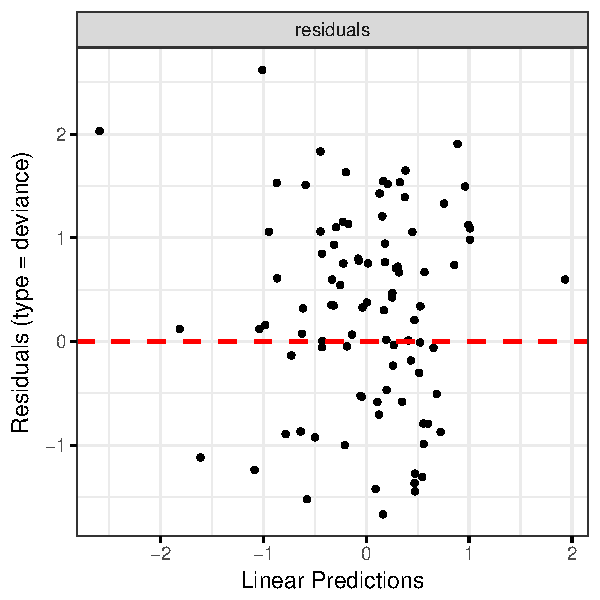
\includegraphics{fig/phreg_residuals.pdf}
  \caption{\label{fig:phreg_residuals}\csentence{Proportional hazards model residuals.}
  Deviance residuals versus predicted log-hazard in a model of mouse
  survival that includes all design parameters (site, sex, and treatment)
  as well as the three SCFAs: propionate, butyrate, and acetate.
  }
\end{figure}

While regression coefficients can be directly interpreted as a proportional
increase or decrease in hazard of death at all time points, in the general
case, this does not equate to a proportional change in expected survival time.
It can therefore be challenging to understand the magnitude of the survival
effect on expected lifespan.
To provide a more intuitive demonstration of the size of the effect,
we compared predicted survival curves for ACA treated, male mice
at UM, with different SCFA concentrations characteristic of two existing
individuals, based on a hypothetical
scenario in which mice were alive at 830 days of age (i.e.~a conditional
expected survival curve; see Fig.~\ref{fig:survival_predict}).
These simulated results demonstrate the strength of the association between
SCFAs and survival over observed differences in concentrations.

\begin{figure}[h!]
  \centering
  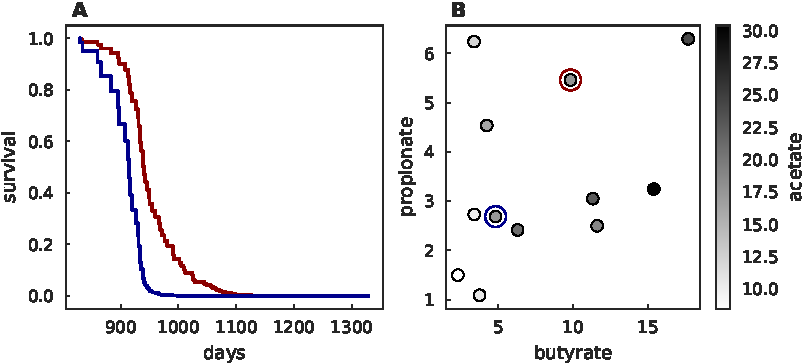
\includegraphics{fig/survival_predict.pdf}
  \caption{\label{fig:survival_predict}\csentence{Effects of SCFAs on longevity.}
  Predicted survival of mice exhibiting realistic variation in SCFA
  concentrations.
  (A) Expected survival curves for male, ACA treated mice at UM, conditional
  on being alive at 830 days of age, and (B) SCFA concentrations for that same
  set of mice.
  Two representative butyrate, propionate, and acetate concentrations were chosen
  to match the measured concentrations for a high (red) and low (blue)
  butyrate/propionate individual, both having similar acetate concentrations.
  }
\end{figure}

\FloatBarrier

%%%%%%%%%%%%%%%%%%%%%%%%%%%%%%%%%%%%%%%%%%%%%%
%%                                          %%
%% Backmatter begins here                   %%
%%                                          %%
%%%%%%%%%%%%%%%%%%%%%%%%%%%%%%%%%%%%%%%%%%%%%%

\begin{backmatter}

\section*{List of abbreviations}

\textbf{ACA:}                  Acarbose
\textbf{SCFA:}                 Short-chain fatty acid
\textbf{ITP:}                  Interventions Testing Program
\textbf{TJL:}                  The Jackson Laboratory
\textbf{UM:}                   The University of Michigan
\textbf{UT:}                   The University of Texas Health Science Center at San Antonio
\textbf{OTU:}                  Operational taxonomic unit
\textbf{HPLC:}                 High-performance liquid chromatography
\textbf{LASSO:}                Least absolute shrinkage and selection operation
\textbf{\taxon{S.~alaskensis}:} \taxon{Sphingopyxis~alaskensis}
\textbf{FDR:}                  False-discovery rate
\textbf{PBS:}                  Phosphate-buffered saline

\section*{Ethics approval and consent to participate}

All mice used in this study were maintained in specific-pathogen free
conditions, and the protocols for husbandry and experimentation were approved
by the Institutional Animal Care and Use Committees at each of the three
institutions.

\section*{Availability of data and materials}

The sequence datasets generated and analyzed during the current
study have been uploaded to the SRA database, accession SRP136736.
Full-cohort survival data analyzed for portions of this study are
available from the corresponding author on reasonable request.
Code and metadata needed to reproduce the processing of raw data and downstream
analyses is available at \url{https://github.com/bsmith89/smith2018paper}.

\section*{Competing interests}

The authors declare that they have no competing interests.

\section*{Funding}

This research was supported by National Institute of Health grants
U01-AG022303 (RAM), U01-AG022308 (DEH), and U01-AG022307 (RS),
The Glenn Foundation for Medical Research (TMS),
the Host Microbiome Initiative at the University of Michigan and
an Integrated Training in Microbial Systems fellowship (BJS).

\section*{Author's contributions}

DEH, RS, and RAM are principal ITP investigators at the three collaborating
institutions and are responsible for design of the mouse experiment and
supervision of technical personnel.
ACE assembled and analyzed preliminary data.
BJS collected the microbiome data and interpreted it along with TMS and RAM\@.
BJS wrote a majority of the manuscript with contributions from TMS and RAM, who
also helped with editing the manuscript.
All authors read and approved the contents of the final article.

\section*{Acknowledgments}

% TODO: Check with acknowledgees

We would like to thank Marian Schmidt, Nicole Koropatkin, Anna Seekatz, Nielson
Baxter, Clive Waldron,
and members of the Schmidt Lab for feedback.
We appreciate the technical support at each of the study sites for maintaining
the animals and collecting the samples.



%%%%%%%%%%%%%%%%%%%%%%%%%%%%%%%%%%%%%%%%%%%%%%%%%%%%%%%%%%%%%
%%                  The Bibliography                       %%
%%                                                         %%
%%  Bmc_mathpys.bst  will be used to                       %%
%%  create a .BBL file for submission.                     %%
%%  After submission of the .TEX file,                     %%
%%  you will be prompted to submit your .BBL file.         %%
%%                                                         %%
%%                                                         %%
%%  Note that the displayed Bibliography will not          %%
%%  necessarily be rendered by Latex exactly as specified  %%
%%  in the online Instructions for Authors.                %%
%%                                                         %%
%%%%%%%%%%%%%%%%%%%%%%%%%%%%%%%%%%%%%%%%%%%%%%%%%%%%%%%%%%%%%

% if your bibliography is in bibtex format, use those commands:
\bibliographystyle{doc/template/bmc-mathphys} % Style BST file (bmc-mathphys, vancouver, spbasic).
\bibliography{doc/bibliography.bib}      % Bibliography file (usually '*.bib' )
% for author-year bibliography (bmc-mathphys or spbasic)
% a) write to bib file (bmc-mathphys only)
% @settings{label, options="nameyear"}
% b) uncomment next line
%\nocite{label}

% or include bibliography directly:
% \begin{thebibliography}
% \bibitem{b1}
% \end{thebibliography}

%%%%%%%%%%%%%%%%%%%%%%%%%%%%%%%%%%%
%%                               %%
%% Tables                        %%
%%                               %%
%%%%%%%%%%%%%%%%%%%%%%%%%%%%%%%%%%%

% No tables are larger than one page, so we don't put them at the end.
%% Use of \listoftables is discouraged.
%%
% \section*{Tables}
% \begin{table}[h!]
% \caption{Sample table title. This is where the description of the table should go.}
%       \begin{tabular}{cccc}
%         \hline
%            & B1  &B2   & B3\\ \hline
%         A1 & 0.1 & 0.2 & 0.3\\
%         A2 & ... & ..  & .\\
%         A3 & ..  & .   & .\\ \hline
%       \end{tabular}
% \end{table}

%%%%%%%%%%%%%%%%%%%%%%%%%%%%%%%%%%%
%%                               %%
%% Additional Files              %%
%%                               %%
%%%%%%%%%%%%%%%%%%%%%%%%%%%%%%%%%%%

\end{backmatter}
\end{document}
